\UseRawInputEncoding

\documentclass[11pt]{article}
\usepackage{colacl}
\usepackage{graphicx}
\usepackage{caption}
\usepackage{subcaption}
\usepackage{multirow}
\usepackage{natbib}
%\usepackage [latin1]{inputenc}
\graphicspath{ {C:/Users/hugoa/Desktop/Uni/Introduction to Machine Learning/Assignment 3/COMP90049-report-templates/COMP90049-report-template latex/figures/} }
\sloppy



\title{COMP90049 Assignment 3 \\ \textit{Does Self-Training Using Unlabelled Data Improve Job Salary Classification?}}
\author
{Anonymous}



\begin{document}
\maketitle

\section{Introduction}

Predicting the expected salary for a job based on its description 
is something many job seekers could benefit from, and the 
problem sits neatly in the domain of Natural Language Processing.

We are faced with a dataset of labelled and 
unlabelled job descriptions with the task of predicting their salaries.
I have implemented semi-supervised Logistic Regression (LR), 
k-Nearest Neighbours (KNN), and Multinomial Naive Bayes (MNB) models 
to ascertain whether the inclusion of unlabelled data in self-training improves job salary prediction.


\section{Literature Review}

Job salary prediction in prior works has been based on a variety of features, 
sourced from both job posting platforms and companies \citep{Samah2022}\citep{Martin2018}\citep{Bhola2020}\citep{Demir2022}.
Commonly used attributes include the job title, textual description, 
required qualifications and experience, company, location, time dedication, 
and company focused features such as number of employees, 
industry sectors, and gross product. 

Most approaches involve transformation of textual features into a smaller numerical feature space. \citet{Bhola2020} achieve strong results through encoding textual job descriptions 
by mapping them to embeddings, resulting in a feature space of fewer dimensions, 
with real-valued feature values associating word contextual meaning.
They apply this in a binary one-vs-rest model for predicting a large sized label set of job skills. 

For the prediction of opening weekend movie revenue,  \citet{Joshi2010} retain the textual nature of features, and 
limits features through partitioning complex words/phrases, 
parts-of-speech, and dependency triplets. Their results support 
the use of textual features rivalling that of metadata in the prediction of the real-valued targets.

\citet{Liu2020} use news headlines as term frequency-inverse document frequency (TF-IDF) 
vectors as well as word embedding to predict stock market movement, 
showing a higher performance using embeddings for machine learning algorithms.

In early semi-supervised works, \citet{Yarowsky1995} shows great success in 
word sense disambiguation using minimally one seed collocation for each 
word sense in the form of a common adjacent word. Even in these contexts of 
little to no labelled training data their algorithm matches or outperforms comparable supervised algorithms. 

In this paper, I employ LR, KNN, and 
MNB models with both word-embeddings and TF-IDF job 
descriptions to assess the value of unlabelled data in the prediction of job salaries.

\section{Method}

\subsection{Data}

The data, derived and made available by \citet{Bhola2020}, consists of a total of 9,738 labelled and 5,902 unlabelled instances, 
out of which 1,738 labelled instances are partitioned as a validation set. 
Finally, another 1,737 unlabelled job descriptions are provided as a test set, 
against which prediction accuracy can be checked through the Kaggle competition.

Job descriptions are transformed using word embeddings and TF-IDF, 
with the former used for LR and KNN models, and the latter for MNB. 
Embeddings are computed by a pre-trained sentence transformer that 
integrates the language model from \citet{Reimers2019}, and 
result in 384-dimensional vectors that are associated with the contextual meaning 
of words in the job description. TF-IDF vectors are built on the frequency of 
the words in the instance alongside the inverse word frequency across 
the dataset, resulting in higher values for words highly relevant to a 
particular job description. The TF-IDF data has had stop words removed and is 
limited to the words with the top 500 values \citep{Shutze2008}.

For comparison against the KNN model, the target salary labels have been 
partitioned into 10 equal-frequency bins ranging 0-9 used as the targets for all tested models.

%Text of the subsection with citations such as 
%\newcite{Spa72}, \newcite{Kay86} and \newcite{MosWal64}.
%Note that the citation style is defined in the accompanying
%style file; it is similar to AAAI house style. You may use
%other (formal) citation styles if you prefer.

 
\subsubsection{Models}

For this task I have chosen LR, KNN, and MNB models to gain a variety of 
results with which to explore my research question and also compare the 
relative effect of unlabelled data on the different models and their assumptions.

A key difference between LR and MNB is that the latter assumes that 
features are independent conditional on the class. In the domain of NLP, this 
seems unintuitive, however NB is known to nevertheless perform well. 
Both of these models make assumptions about the distribution of the data, 
which may not match reality. In comparison, KNN makes no assumptions 
about the distribution of input data. Additionally, the use of embeddings 
allows us to compute the distance between job descriptions of similar ``meaning'', which is ideally suited to KNN.

\subsection{Evaluation Metrics}
 
\begin{itemize}
	\item \textbf{Baselines}: Inherent to the research question, fully supervised versions of the same models used make up the most relevant baseline. We can also note that due to the equal frequency binning, a Zero-R Classifier achieves an accuracy of $\approx10\%$.
	\item \textbf{Accuracy}: the proportion of correct predictions. This is the only available metric given for predictions made against the test set, and is hence used with precedence.
	\item \textbf{$F_1$ Score}: a balanced representation of both precision and recall. Precision is the proportion of true positive predictions averaged across labels. Recall is the proportion of positive predictions out of actual positives for that label averaged across labels 
	\item \textbf{Qualitative}: I also assessed whether the reportedly best confidence thresholds in self-training are of an acceptable level in respect to their value and the number of selected instances.
\end{itemize}

\section{Implementation \& Results}

For each model, selection of the optimal data set representation (embeddings or TF-IDF) and calibration of model parameters was carried out before moving on to self-training.
The models were first trained on the labelled training data, using both the embedded and TF-IDF data, and tested against the validation set using a range of parameters. 

In our final results, the embedded data is used for LR and KNN, whilst MNB utilises the TF-IDF data. 
This results in a gap of comparability between the two sets, but importantly does not hinder the 
answering of the main research question, which in this case is more greatly concerned with comparison between the models' supervised and semi-supervised variants.
The ideal parameters determined are shown in Table~\ref{table:params}.


\begin{table}[h]
 \begin{center}
\begin{tabular}{|l||l|c|}

      \hline
      \textbf{Model} & \textbf{Parameter} & \textbf{Value}\\
      \hline\hline
      LR & Max iterations & 250\\
	\hline
      \multirow{2}{4em}{KNN} & Distance metric & cosine\\
       & \textit{K} & 20\\
	\hline
      MNB & $\alpha$ & 0.7\\
      \hline

\end{tabular}
\caption{Tuned model parameters}
\label{table:params}
\end{center}
\end{table}

Self-training was implemented using Scikit-learn SelfTrainingClassifier \citep{sklearn}, which utilises bootstrapping.

Given sets of labelled and unlabelled data, the base classifiers (our models) are trained on the 
labelled set, and then iteratively add unlabelled instances that have predictions with 
high confidence to the labelled set with pseudo-labels, and retrain the model on 
this augmented labelled data. High confidence is defined by a pre-set threshold 
parameter that remains constant for iterations; iterations stop upon reaching a 
limit or finding no instances with predictions that meet the threshold. 
The ability of a model to produce some confidence value of a 
prediction is essential for this process, a criterion that our selected models meet.

All labelled (8,000) and unlabelled (5,902) training data 
available were used to implement this LR, KNN, and MNB models, with a 
range of confidence thresholds. Due to needing to submit to Kaggle to get 
results for predictions on the test set, these were tested on the validation set for comparison, prior to submission. 
Prediction accuracy on the validation set using the self-trained models with 
varying thresholds is shown in Figures~\ref{fig:self LR},~\ref{fig:self KNN}, and~\ref{fig:self MNB}, 
and, based on the best threshold shown, Table~\ref{table:self test} shows the accuracy achieved on the test set (submitted to Kaggle).

\begin{figure}[h]
\caption{Self-Training Models}
\begin{subfigure}{0.5\textwidth}
	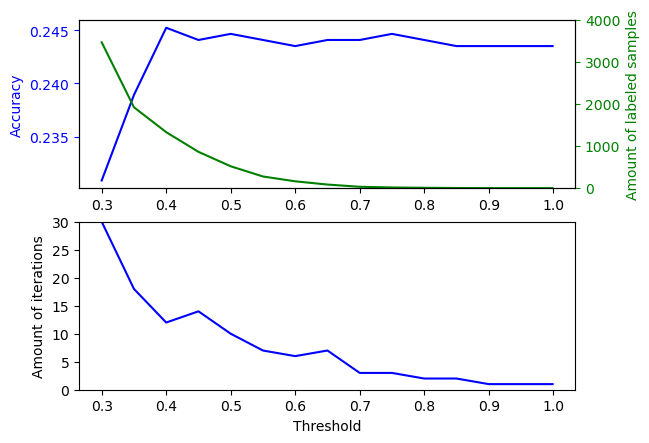
\includegraphics[width=\textwidth]{self_LR_thresholds_graph.png}
	\caption{Self-Training Logistic Regression}
	\label{fig:self LR}
	\centering
\end{subfigure}	
\begin{subfigure}{0.5\textwidth}
	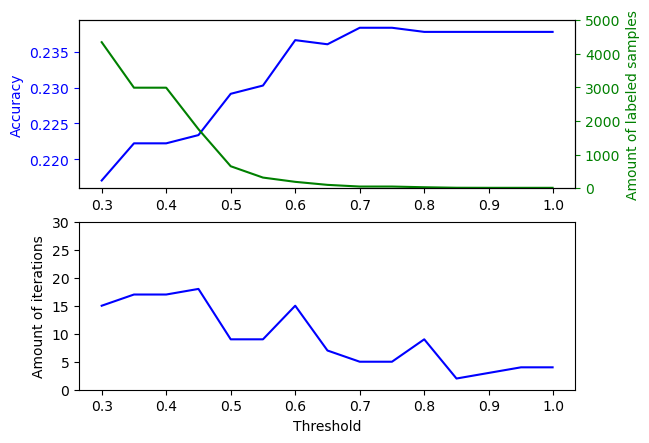
\includegraphics[width=\textwidth]{self_KNN_thresholds_graph.png}
	\caption{Self-Training \textit{K}-Nearest Neighbours}
	\label{fig:self KNN}
	\centering
\end{subfigure}
\begin{subfigure}{0.5\textwidth}
	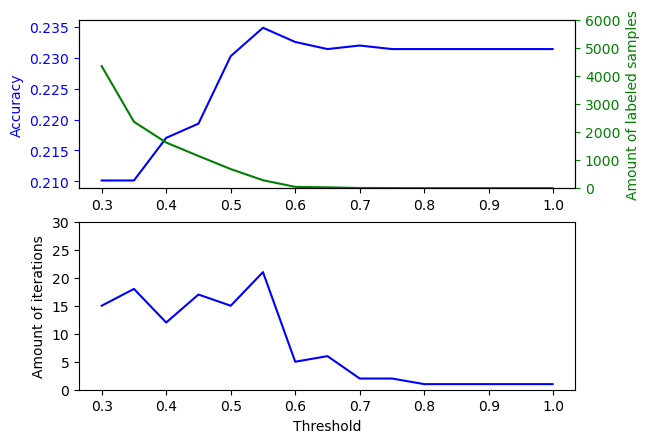
\includegraphics[width=\textwidth]{self_MNB_thresholds_graph.png}
	\caption{Self-Training Multinomial Naive Bayes}
	\label{fig:self MNB}
	\centering
\end{subfigure}

\end{figure}

\begin{table}[h]
 \begin{center}
\begin{tabular}{|l||c|c|}

      \hline
      \textbf{Model} & \textbf{Threshold} & \textbf{Accuracy}\\
      \hline\hline
      LR & 0.75 & 0.2438\\
	\hline
      KNN & 0.75 & 0.2188\\
	\hline
      MNB & 0.70 & 0.2246\\
      \hline

\end{tabular}
\caption{Self-training accuracy on test set}
\label{table:self test}
\end{center}
\end{table}

\vspace{3mm}
Due to the importance of the prediction confidence or probability estimates from our models, 
a further step was taken in calibrating the models to optimise this. 
Without this, confidence estimates from our models do not necessarily map 1:1 with 
the implied probability of belonging to a class. By applying Scikit-learn CalibratedClassifierCV, 
these probability estimates will be consistently indicative of prediction confidence. 
The specific calibration was conducted using a one-vs-rest isotonic regressor.
This process is expected to improve self-training performance as our chosen thresholds will be more 
accurately abided by, and comparison between model prediction confidence will be consistent. 

Calibration was done on fresh models, using the same labelled and unlabelled training data. 
Cross-validation is used to repeatedly split this input data into inner train and test sets, 
from which final prediction probability estimates derived as averages across the iterated models. 

For the same reason as stated above for the uncalibrated self-training models, these were tested on the validation set first.
Figures~\ref{fig:cal self LR},~\ref{fig:cal self KNN}, and~\ref{fig:cal self MNB} show threshold results for the calibrated self-training models, and 
Table~\ref{table:cal self test} shows the best threshold accuracy on the test set.

\begin{figure}[h]
\caption{Calibrated Self-Training Models}
\begin{subfigure}{0.5\textwidth}
	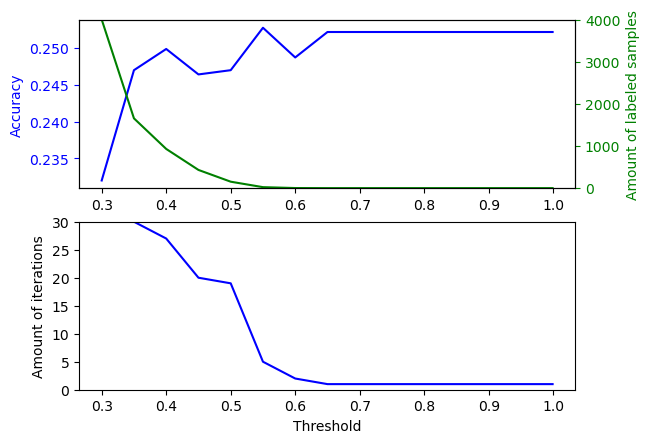
\includegraphics[width=\textwidth]{iso_self_LR_thresholds_graph.png}
	\caption{Calibrated Self-Training Logistic Regression}
	\label{fig:cal self LR}
	\centering
\end{subfigure}	
\begin{subfigure}{0.5\textwidth}
	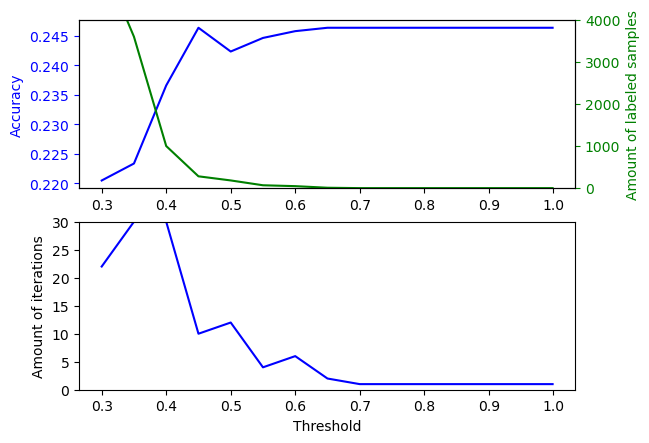
\includegraphics[width=\textwidth]{iso_self_KNN_thresholds_graph.png}
	\caption{Calibrated Self-Training \textit{K}-Nearest Neighbours}
	\label{fig:cal self KNN}
	\centering
\end{subfigure}
\begin{subfigure}{0.5\textwidth}
	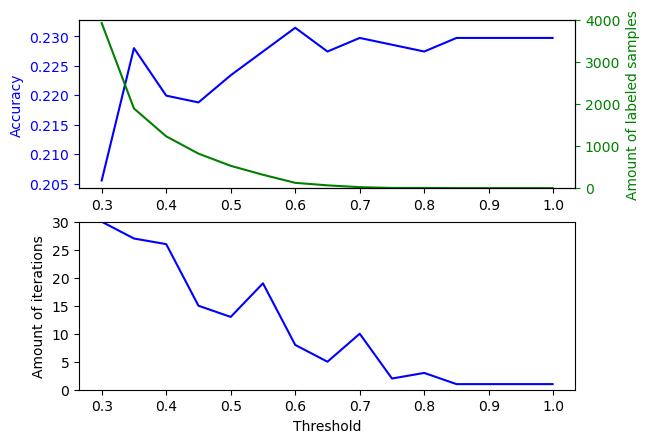
\includegraphics[width=\textwidth]{iso_self_MNB_thresholds_graph.png}
	\caption{Calibrated Self-Training Multinomial Naive Bayes}
	\label{fig:cal self MNB}
	\centering
\end{subfigure}

\end{figure}

\begin{table}[h]
 \begin{center}
\begin{tabular}{|l||c|c|}

      \hline
      \textbf{Model} & \textbf{Threshold} & \textbf{Accuracy}\\
      \hline\hline
      LR & 0.55 & 0.2399\\
	\hline
      KNN & 0.55 & 0.2226\\
	\hline
      MNB & 0.60 & 0.2131\\
      \hline

\end{tabular}
\caption{Calibrated self-training accuracy on test set}
\label{table:cal self test}
\end{center}
\end{table}

\section{Discussion}

As can be seen, results against the validation data are underwhelming with little to no difference in 
performance when comparing the calibrated semi-supervised models with their baseline supervised versions. 
Of the final calibrated self-training models, LR and KNN both show a gain of 0.009 accuracy when predicting the validation set, and a slight loss in $F_1$ score. Against the test set, accuracy \textit{decreased} for both the LR and MNB models, and showed a marginal improvement for only KNN.
There are several reasons that this might be the case.

A possible explanation for this is that prior to training on the unlabelled data, the models have 
already learned the most important relations between the attributes and labels. Checking the performance 
of our baseline supervised models against their training data shows a best accuracy of 0.337, 
not much better than our validation or test predictions. A learning curve defined by 
these features shows high bias, and may explain why additional (unlabelled) data does not help our models.
Semi-supervised learning is commonly employed and most effective when the amount of labelled data available is 
very limited, which isn't the case here. Indeed, training on unlabelled data can result in a decrease in 
performance when adequate labelled data is already in use \citep{Chapelle2006}.

Across each of the models, the general low predictive probabilities may prevent a gradual inclusion of unlabelled instances, 
with only a small number of instances receiving pseudo-labels once predictive probability surpasses 0.5.
With the general low accuracy across our models, it is likely that falsely pseudo-labelled instances cause error propagation at lower confidence thresholds.
In a scenario with few labelled instances available, a threshold approach may not allow the trickling of only the most confidently predicted instances into the labelled data set.
Additionally, as noted by Scikit-learn, isotonic calibration reduces extremes in predictive probabilities \citep{sklearn}. 
We can see that post calibration the number of unlabelled instances chosen by the self-trainer declines 
more steeply as the threshold rises. It is also possible that some previously very low confidence predictions 
have been brought up into the middle-low band of thresholds, further bloating this cohort.
A $K$-best approach to pseudo-labelling instances may achieve better results in these scenarios.

The use of word-embeddings for feature representation prima facie improves peformance in our models over using raw text.
However, this does not mean that the distribution of instances in our 384-dimension feature space is representative of the target classes.
The partitioning of salaries into ten bins is suggestive of an equal number of clusters to be found, however this is not necessarily the case. 

For our purposes of salary prediction based on job description, it is likely that a more complex model would perform better. 
Relationships between job description features and salary is likely not an easy fit to a multinomial distribution, or easily grouped for KNN.
Additionally, whilst feature transformation in the way of TF-IDF and embeddings helps to capture important information in the textual description,
the inclusion of other features related to the job posting may further improve performence, such as required qualifications and experience.
These features could be modified further to be weighted based on their informational value (entropy), or inversely weighted based on their correlation with other features.

\section{Conclusions}
I have explored the prediction of job salary based on job description from supervised and semi-supervised approaches. 
The inclusion of unlabelled data in self-training did not lead to an increase in performance in this scenario using LR, KNN, and MNB models.
I suggest possible reasons for this being the size of the labelled training data set nullifying potential further learning from unlabelled data, 
poor supervised model performance prior to self-training, and the complexity of the problem.

\nocite{*}
\bibliographystyle{apalike}
\bibliography{A3_references}

\end{document}
